\chapter{Solute diffusion in solids}

\section{Solid state diffusion}

We consider a few simple cases of solid state diffusion.

\subsection{Steady state diffusion profiles}

Consider the phase diagram to arrive at the interface compositions during diffusion couple experiments. The case of intermediate metastable phase with and without the possibility of it's nucleation. 

\subsection{Fixed boundary compositions}

In the domain, composition is fixed with the following boundary conditions:\\
$C = C_s$ at $x = 0$ and $t > 0$\\
$C = C_\infty$ at $x = \infty$ \\
$C = C_s$ at $t = \infty$ and $x > 0$\\

The governing equation is $$ {\partial C \over \partial t} = D {\partial^2 C
\over \partial x^2} $$

By using a variable substition $\eta = {x \over 2 \sqrt{Dt}}$, one can integrate
the equation subject to the above boundary conditions as:

$$ {C - C_\infty \over C_s - C_\infty} = 1 - \text{erf} {x \over 2 \sqrt{Dt}} =
\text{erfc} {x \over 2 \sqrt{Dt}}$$

\begin{figure}[h]
\begin{center}
\framebox{
 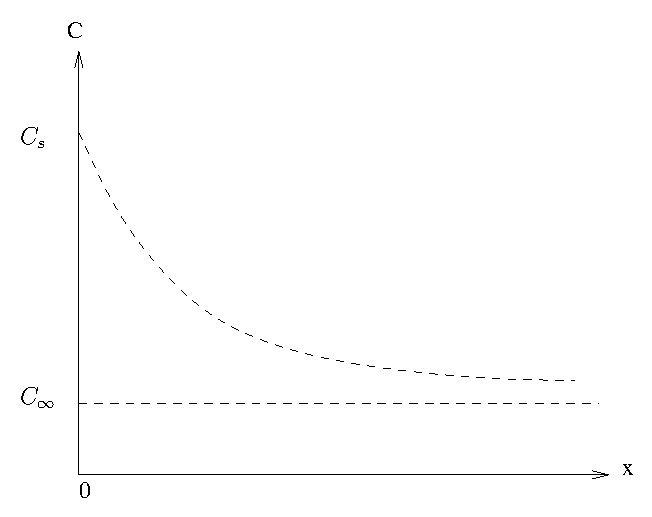
\includegraphics[scale=0.7]{images/c20-fixcompfig.ps}
}
\end{center}
\caption{Fixed Compositions}
\label{slab}
\end{figure}

\subsection{Fixed total solute content}

In the domain, the total solute is fixed with the following boundary
condition:\\
$$ \int_{-\infty}^{\infty}{C dx} = M$$

The governing equation to be solved is same as Fick's second law of solute
diffusion. In order to figure out the form of $C$ that will satisfy the
governing equation as well as the boundary condition, we use the property of
erf(x).

$$ \text{erf} (\infty) = 1 = {2 \over \sqrt{\pi}} \int_{0}^{\infty}{\exp(-{x^2
\over 4Dt}) {1 \over 2 \sqrt{Dt}} dx}$$

Using algebraic manipulations,

$$ \int_{-\infty}^{\infty}{ {M \over 2 \sqrt{\pi D t}} \exp(-{x^2 \over 4Dt})
dx} = M = \int_{-\infty}^{\infty}{C dx}$$

One can verify that the following form of solution for $C$ will not only satisfy
the boundary condition as given above but also the governing equation.

$$ C = {M \over 2 \sqrt{\pi D t}} \exp(-{x^2 \over 4Dt}) $$


\subsection{Fourier series solution}

In this section we describe the Fourier series solution of diffusion equation and its application in Homogenization heat treatment process.

\subsection{Diffusion during growth of precipitate}

Zener's solution, Role of curvature on the interface composition, ...

\subsection{Solute profile during directional solidification}

During directional solidification, one can consider solute balance at the solid-liquid interface as follows. The solute dumped into the liquid by the growing solid due to solute partition effect is taken away into the bulk liquid by diffusion. The liquid composition is then given as a function of distance from the solid-liquid interface as follows:

\begin{equation}
{C_l \over C_0} = 1 + {1-k\over k} \exp{\left(- {Vx \over D}\right)}
\end{equation}

Here, $k$ is the partition coefficient, $V$ is the velocity of the solid-liquid interface, $D$ is the diffusivity of the solute in the liquid and $C_0$ is the initial / steady-state solute concentration.

\subsection{Solute profile during eutectic solidification}

Here we talk about Jackson-Hunt's solution

\section{Diffusion with two species considered}

\subsection{Interdiffusion coefficient}

Here we derive the expression for interdiffusion coefficient $\tilde{D}$ for the case of constant density.

\subsection{Stagnant layer approach}

\begin{figure}[h]
\begin{center}
\framebox{
 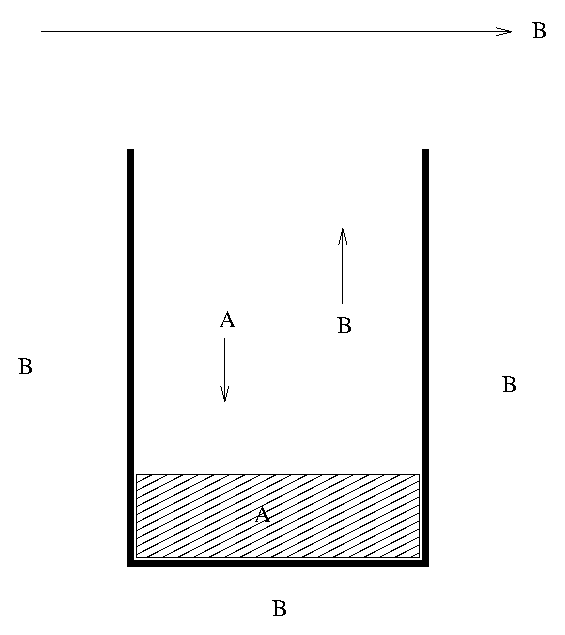
\includegraphics[scale=0.7]{images/c20-stagnantfig.ps}
}
\end{center}
\caption{Stagnant layer approach}
\label{stagnant}
\end{figure}

Consider a situation such as in the figure \ref{stagnant}. At the bottom layer,
species A is being generated and we are interested in the net flux of A and its
distribution in the layer above. It can be taken that in the stagnant layer,
there is no net flux of B. 
The net flux equations are:

$$ j_A = -D_{AB} {\partial \rho_A \over \partial x} + u \rho_A $$
$$ j_B = -D_{AB} {\partial \rho_B \over \partial x} + u \rho_B = 0$$
or
$$ u = { D_{AB} \over \rho_B} {\partial \rho_B \over \partial x}$$

If only species A and B are present and the total density $\rho$ is constant,

$$ \rho_A + \rho_B = \rho$$
such that 
$$ {\partial \rho_B \over \partial x} = - {\partial \rho_A \over \partial x}$$

Substituting in the equation of net flux of A,

$$ j_A = -D_{AB} {\partial \rho_A \over \partial x} - \rho_A {D_{AB} \over (\rho - \rho_A) }
{\partial \rho_A \over \partial x} $$

$$ j_A =  - D_{AB} {\rho \over (\rho - \rho_A)} {\partial \rho_A \over \partial x} $$

At steady state, 

$$ \vec{\nabla} \cdot {\vec{j_A}} = 0$$

or

$$ {\partial \over \partial x} \left[ {\rho \over (\rho - \rho_A)} {\partial \rho_A \over
\partial x} \right] = 0 $$

Integrating twice with the boundary conditions:

\begin{itemize}
\item Considering that species B is being flushed at the top, concentration of
species A at $x=L$, the height of the layer can be taken as $\rho_{AL}$, usually
zero. 
\item At $x=0$, $\rho_A = \rho_{A0}$
\end{itemize}

we obtain the solution for distribution of $\rho_A$ in the stagnant layer as:

$$ \boxed{
\ln {\rho - \rho_{A} \over \rho - \rho_{A0}} = {x \over L} \ln {\rho - \rho_{AL} \over \rho - \rho_{A0}}
}$$

Using the above expression,

$$ {\partial \rho_A \over \partial x} = - { (\rho - \rho_A) \over L } \ln {\rho - \rho_{AL}
\over \rho - \rho_{A0}} $$

Substiting the same to obtain $j_A$,

$$ \boxed{
j_A = {D_{AB} \rho \over L} \ln {\rho - \rho_{AL} \over \rho - \rho_{A0}} 
}$$

In the limit of $\rho_{A0} = 0$ and the value of $\rho_{AL}$ being small, the above
equation reduces to $j_A = -D_{AB} {\rho_{AL} \over L}$, which is the same as
Fick's first law valid for the case of no advection. Thus, the stagnant layer
approach with very dilute species can be approximated to the regime where Fick's
law is applicable even though the other species is also taking part in the
diffusion process.

It is easy to see that instead of concentrations, if one were to use partial
pressures of the respective species, one would have the following  equations
valid:

$$p_A + p_B = p$$

$$p_A = RT C_A$$

$$ \ln {p - p_A \over p - p_{A0}} = {x \over L}  \ln {p - p_{AL} \over p -
p_{A0}} $$

$$ j_A = {p D_{AB} \over RTL} \ln {p - p_{AL} \over p - p_{A0}}$$

$j_A$ when expressed in rate of loss of mass can be accuarately measured and
thus provides an excellent means to obtain $D_{AB}$ by weight loss method using
a setup similar to that of figure \ref{stagnant}.



\section{Boundary conditions}

In most of the cases, the diffusion within the domain can be simplified to be one dimensional and be solved either using the solid state diffusion equation or stagnant layer approach. However, the conditions at the boundary of the domain are required in all cases. Following are few ways to obtain those boundary conditions.

\subsection{Solubility limts}

In situations such as carburising / decarburising and nitriding, the maximum concentration of the corresponding species in the domain at the boundary can be obtained by looking up the phase diagram. The solid solution limits can be used as boundary conditions.

\subsection{Reaction mass transfer}

In a reaction, we are interested in the rate of formation of a particular
product, usually a condensed one. It can usually be obtained by knowing the flux
of that species by balacing with the flux of a diffusing species and applying
appropriate boundary conditions. The compositions of the participating species
are related by the equilibrium constant of the reaction. Consider the following
example.

$$ A_{(g)} \rightarrow n B_{(g)} + C_{(s)} $$

$$ K = { [B]^n \over [A] } = {p_B^n \over p_A} $$
$$ p_A + p_B = p$$

One can solve for $p_B$ by solving the above two equations.

One has to know the value of $K$ at a given temperature and should watch out the
units of $K$ to know the convention for the units of $[A]$ and $[B]$.

Once the value of $K$ is known, it is possible to obtain the flux of one of the
species, say A, using either the Fick's law or the stagnant layer approach
depending on how dilute the system is. The fluxes of the diffusing species A and
B are related to as:

$$ j_B = n j_A = n j_C$$

If B is a dilute species in a stagnant layer of A of height $L$ and a total
pressure $p$, one can use the following expression for $j_B$

$$ j_B = {p D_{AB} \over RTL} \ln {p - p_{BL} \over p - p_{B0}}$$

The quantity $j_C$ can then be converted to appropriate rate of formation as
mass or volume or moles or thickness as desired using the properties of $C$.

\subsection{Sieverts Law}

Most of the time, one is interested in determining flux of a species as a
function of the concentration of that species.

\textbf{Sievert's Law} For absorption of gases in metals, one can use the
following expression to obtain the concentration.


$$ {1 \over 2} H_2 \rightarrow [H]$$

Equilibrium constant is given by 

$$ K = { [H] \over \sqrt{p_{H_2}} } $$

If the concentration of hydrogen is given in ppm and the partial pressure in
atm, then K would be in ppm/$\sqrt{\text{atm}}$. One must watch the units of $K$
to know the convention followed. This is because pressure could be in units such
as bar (atm), torr (mmHg), mbar or Pa.

Conversion of partial pressure of a gas into concentration is done by
approximating the gas to be an ideal gas.


$$ p_A V = n_A R T$$

$$ C_A = {n_A \over V} = {p_A \over RT}$$

Here, $C_A$ is given in mol/vol and may need to be converted to mass/vol using
molar weight and density.

